% !TEX root = Kreisfahrt.tex
\section{Mathematische Modellierung}
\begin{figure}
    \centering
    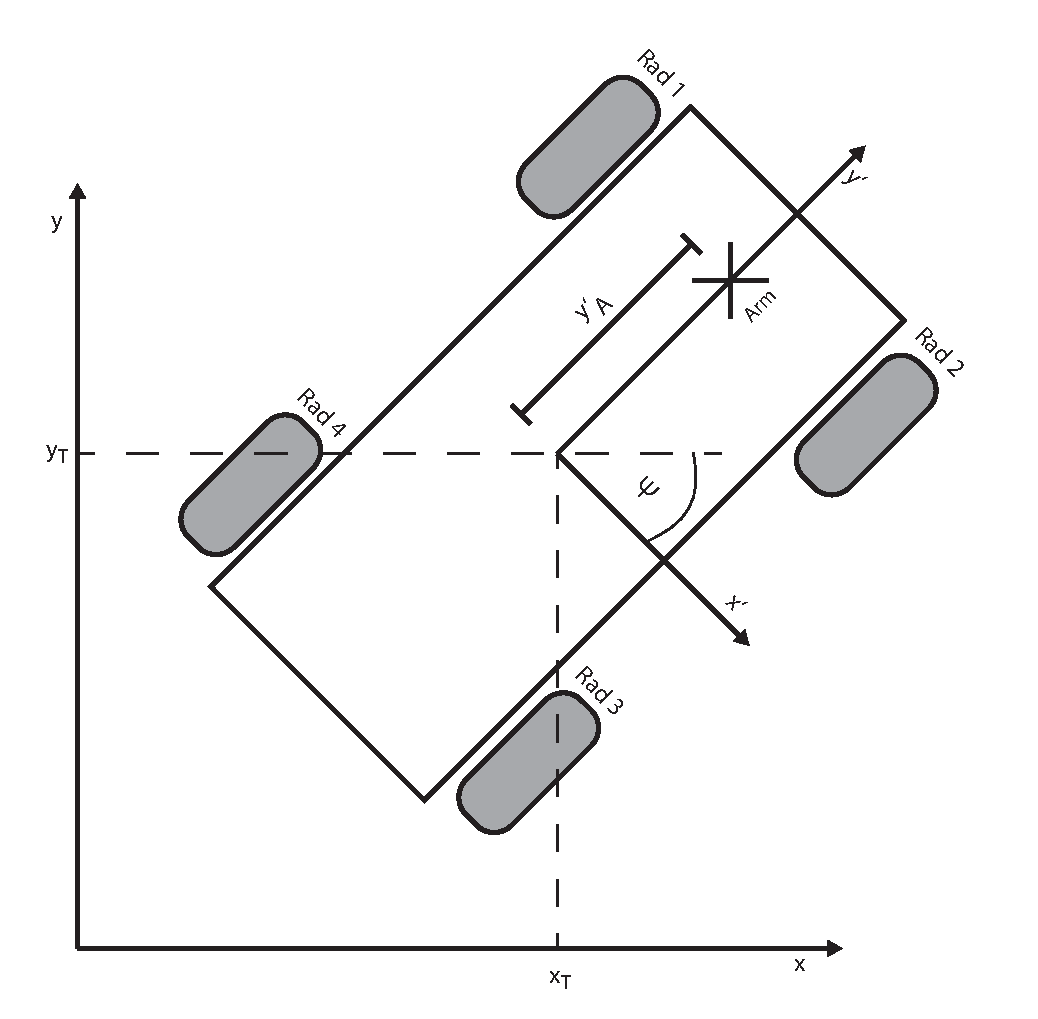
\includegraphics[width=.8\textwidth]{Abbildungen/Koordinaten}
    \caption{Einführung der verwendeten Koordinatensysteme, der Position des Arms sowie der Radnummerierung.}
\end{figure}
Dieses Kapitel beschreibt die Mathematik hinter der Kinematik und Dynamik des Mecanum-Roboters.
Jede Bewegung setzt sich aus einer translatorischen und einer rotatorischen Teilbewegung zusammen.

\subsection{Translation}
Um eine translatorische Bewegung auszuführen, werden die Räder paarweise (1+3, 2+4) mit gleicher Drehrichtung und Drehgeschwindigkeit angetrieben.
Die resultierende Gesamtkraft bestimmt die Richtung der Fahrt.
Die folgenden Rechnungen behandeln die Ermittlung der einzelnen Soll-Radgeschwindigkeiten aus einem vorgegebenen Geschwindigkeitsvektor.

\begin{figure}[H]
    \centering
    \includegraphics[width=.6\textwidth]{Abbildungen/Kraefte-am-Rad}
    \caption{Kräftegleichgewicht an einem Mecanum-Rad.}
\end{figure}

Die Leistung einer vektoriellen Kraft berechnet sich nach:
$$ P_F = F_T \cdot v_F $$

Wirken Kraft und Geschwindigkeit entlang einer Koordinatenachse, haben beide Vektoren die gleiche Komponente ungleich null und ihr Skalarprodukt kann vereinfacht als Produkt der skalaren Größen betrachtet werden.

Die Kraftvektor in $x$- und $y$-Richtung setzt sich zusammen als die Summe der einzelnen $x$- und $y$-Vektoren der vier Räder:
\begin{align*}
    \sum_{i=1}^4 F_{ix} &= \sum_{i=1}^4 F_i \cos \alpha \\
    &= \sum_{i=1}^4 (-1)^i SIG \cdot K_i F_{Ti} \sin \alpha \cos \alpha \\
    &= \sum_{i=1}^4 (-1)^i SIG \cdot \frac{1}{2} K_i F_{Ti}
\end{align*}
\begin{align*}
    \sum_{i=1}^4 F_{iy} &= \sum_{i=1}^4 F_i \sin \alpha \\
    &= \sum_{i=1}^4 SIG \cdot K_i F_{Ti} \sin^2 \alpha \\
    &= \sum_{i=1}^4 SIG \cdot \frac{1}{2} K_i F_{Ti}
\end{align*}

SIG sei die Vorzeichenkonventionen für die Drehrichtung der Räder.
Diese wird in der Steuerung direkt implementiert und wird daher bei den folgenden Rechnungen nicht weiter betrachtet.

Der Winkel $ \alpha $ beschreibt den Winkel, in dem die Rollen auf dem Mecanum-Rad angebracht sind.
In den meisten Fällen gilt $\alpha = 45^\circ$.

Für eine translatorische Bewegung müssen die Radpaare mit gleicher Geschwindigkeit drehen.
Entsprechend müssen ihre Kraftvektoren $F_{T1, 3} / F_{T2, 4}$ gleich groß sein.
Durch Auflösen der Summenzeichen erhält man ein Gleichungssystem:
\begin{align*}
    F_x &= - K_i F_{T1, 3} + K_i F_{T2, 4} \\
    F_y &= K_i F_{T1, 3}   + K_i F_{T2, 4}
\end{align*}

Nach dem Umstellen erhält man $F_{T1, 3}$ und $F_{T2, 4}$ und kann somit auch direkt die Geschwindigkeiten berechnen:
\begin{align*}
    F_{T1, 3} &= \frac{F_y + F_x}{K_i} &\Rightarrow v_{T1, 3} &= \frac{v_y + v_x}{K_i} \\
    F_{T2, 4} &= \frac{F_y - F_x}{K_i} &\Rightarrow v_{T2, 4} &= \frac{v_y - v_x}{K_i} \\
\end{align*}

Der Faktor $K_i$ setzt sich aus unterschiedlichen Einzelfaktoren zusammen, welche die durch das Motormoment erzeugten treibenden Kräfte beeinflussen. $K_i$ wird für den Boden der Werkstatt empirisch ermittelt.


\subsection{Rotation}
Die Rotation des Mecanum-Roboters um sein Zentrum müssen alle Räder mit gleicher Geschwindigkeit drehen, lediglich die Richtung unterscheidet sich.
Für eine Drehung im Uhrzeigersinn drehen beispielsweise Rad 1 und 2 rückwärts, Rad 3 und 4 vorwärts. Allgemein gilt:
\begin{align*}
    v_{ref} &= K_i \cdot r \cdot \omega \\
    v_1 = v_4 &= - v_{ref} \\
    v_2 = v_3 &= + v_{ref}
\end{align*}


\subsection{Koordinatentransformation}
Dieses Kapitel befasst sich mit der Koordinatentransformation vom Koordinatensystem des Mecanum-Roboters zum ortsfesten Bezugskoordinatensystem.

Als Beispiel dient der Positionsvektor des montierten Arms im robotereigenen Koordinatensystem:
$$
\underline a' =
    \begin{pmatrix}
        x'_A \\
        y'_A \\
        0
    \end{pmatrix}
$$

Die Position des Roboter-Mittelpunkts wird durch den Vektor $\underline m$ beschrieben.
$$
\underline m =
    \begin{pmatrix}
        x_T \\
        y_T \\
        0
    \end{pmatrix}
$$

Die Rotationsmatrix $\underline R$ um den Gierwinkel $\Psi$ (Rotation um die $z$-Achse) ist definiert als
$$
\underline R_{\Psi} =
    \begin{bmatrix}
        \cos{\Psi}  & -\sin{\Psi} & 0 \\
        \sin{\Psi} & \cos{\Psi} & 0 \\
        0 & 0 & 1
    \end{bmatrix}
$$

Damit lassen sich die Koordinaten eines Punktes auf dem Roboter durch folgenden Zusammenhang in Koordinaten im Referenzsystem umwandeln:
$$
\underline{a} = \underline{m} + \underline{R_\Psi} \cdot \underline{a'} =
\begin{pmatrix}
    x_T + x'_A \cdot \cos(\Psi) - y'_A \cdot \sin(\Psi) \\
    y_T + y'_A \cdot \cos(\Psi) + x'_A \cdot \sin(\Psi) \\
    0
\end{pmatrix}
$$
